\documentclass[tikz,border=4pt]{standalone}
\usepackage[T1]{fontenc}
\usepackage[sfdefault]{biolinum}
\usepackage{tikz}
\usetikzlibrary{arrows.meta,positioning,calc,shapes.geometric,fit,backgrounds,decorations.pathmorphing}

% --- Nord palette ---------------------------------------------------------
\definecolor{nord0}{HTML}{2E3440}
\definecolor{nord1}{HTML}{3B4252}
\definecolor{nord2}{HTML}{434C5E}
\definecolor{nord3}{HTML}{4C566A}
\definecolor{nord4}{HTML}{D8DEE9}
\definecolor{nord5}{HTML}{E5E9F0}
\definecolor{nord6}{HTML}{ECEFF4}
\definecolor{nord7}{HTML}{8FBCBB}
\definecolor{nord8}{HTML}{88C0D0}
\definecolor{nord9}{HTML}{81A1C1}
\definecolor{nord10}{HTML}{5E81AC}
\definecolor{nord11}{HTML}{BF616A}
\definecolor{nord12}{HTML}{D08770}
\definecolor{nord13}{HTML}{EBCB8B}
\definecolor{nord14}{HTML}{A3BE8C}
\definecolor{nord15}{HTML}{B48EAD}

\tikzset{>={Triangle[length=2.4mm,width=2.0mm]}}

\tikzset{
  spine/.style   = {draw=nord10, fill=nord6, text=nord0, very thick, rounded corners,
                    minimum width=2.6cm, minimum height=0.9cm, font=\bfseries, align=center},
  pass/.style    = {draw, fill=white, text=nord0, rounded corners, thick,
                    minimum width=2.7cm, minimum height=0.62cm, font=\small, align=center, inner sep=2pt},
  gtitle/.style  = {text=nord0, rounded corners, thick, minimum width=2.9cm,
                    minimum height=0.62cm, font=\bfseries\small, align=center},
  arr/.style     = {nord3, very thick, ->},
  elabel/.style  = {font=\footnotesize\itshape, text=nord3, inner sep=2pt},
}

\begin{document}
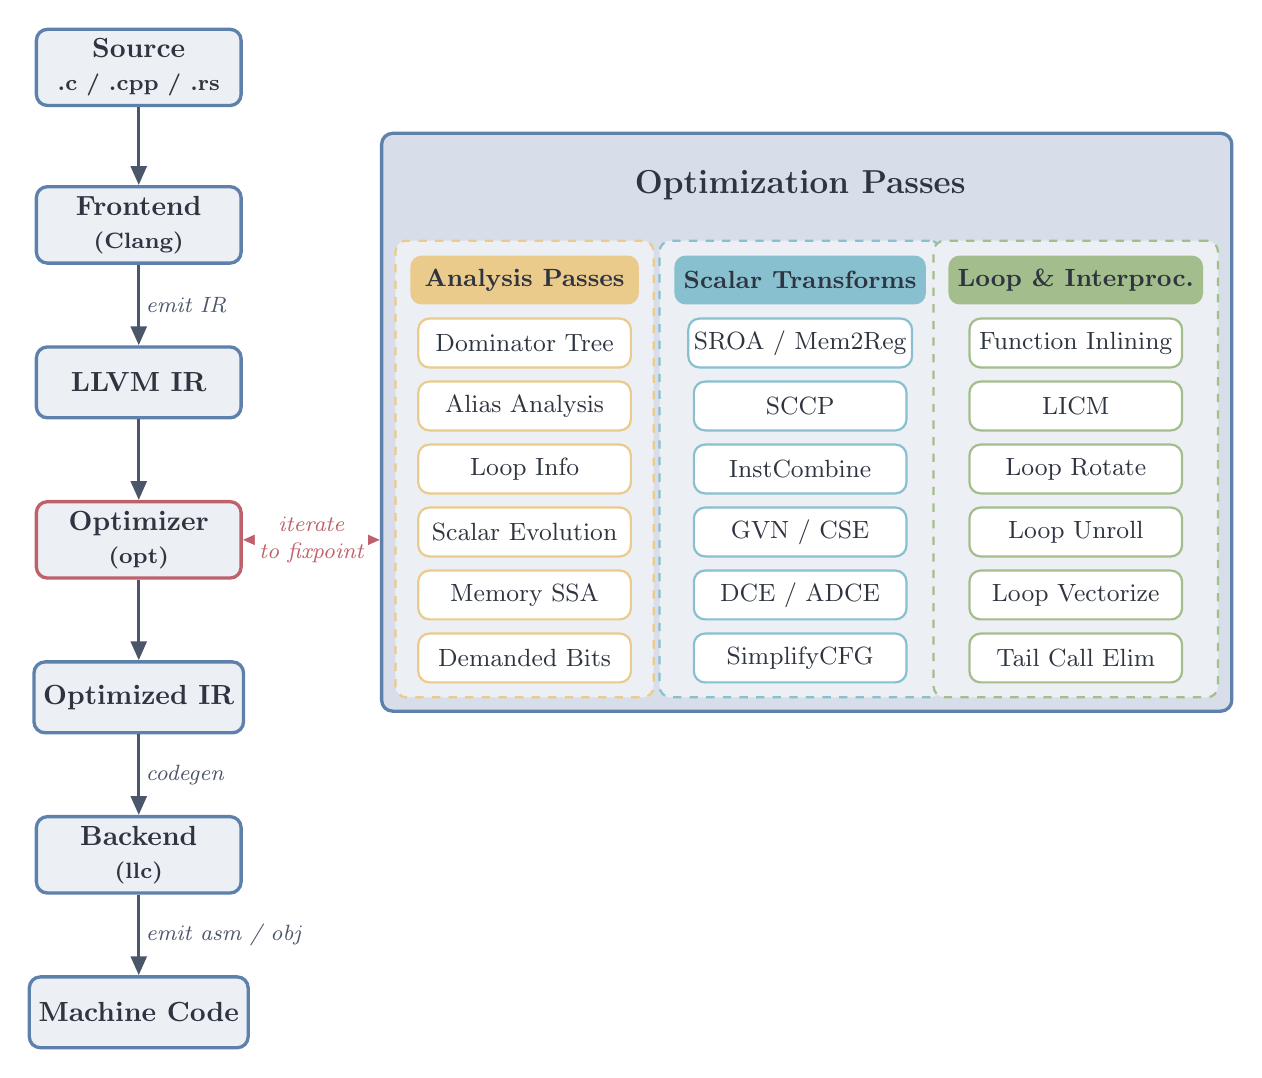
\begin{tikzpicture}

% ---------------- Left spine (main compilation pipeline) ----------------
\node[spine] (src)  at (0,10) {Source\\\footnotesize.c / .cpp / .rs};
\node[spine] (fe)   at (0,8)  {Frontend\\\footnotesize(Clang)};
\node[spine] (ir)   at (0,6)  {LLVM IR};
\node[spine, draw=nord11, very thick] (opt) at (0,4) {Optimizer\\\footnotesize(opt)};
\node[spine] (oir)  at (0,2)  {Optimized IR};
\node[spine] (be)   at (0,0)  {Backend\\\footnotesize(llc)};
\node[spine] (mc)   at (0,-2) {Machine Code};

\draw[arr] (src) -- (fe);
\draw[arr] (fe)  -- node[elabel,right]{emit IR} (ir);
\draw[arr] (ir)  -- (opt);
\draw[arr] (opt) -- (oir);
\draw[arr] (oir) -- node[elabel,right]{codegen} (be);
\draw[arr] (be)  -- node[elabel,right]{emit asm / obj} (mc);

% ---------------- Right panel: optimization passes ----------------
% Column centers
\def\cA{4.9}  \def\cB{8.4}  \def\cC{11.9}
% group titles
\node[gtitle, fill=nord13] (tA) at (\cA,7.3) {Analysis Passes};
\node[gtitle, fill=nord8]  (tB) at (\cB,7.3) {Scalar Transforms};
\node[gtitle, fill=nord14] (tC) at (\cC,7.3) {Loop \& Interproc.};

% Analysis (yellow)
\node[pass, draw=nord13] (a1) at (\cA,6.5) {Dominator Tree};
\node[pass, draw=nord13] (a2) at (\cA,5.7) {Alias Analysis};
\node[pass, draw=nord13] (a3) at (\cA,4.9) {Loop Info};
\node[pass, draw=nord13] (a4) at (\cA,4.1) {Scalar Evolution};
\node[pass, draw=nord13] (a5) at (\cA,3.3) {Memory SSA};
\node[pass, draw=nord13] (a6) at (\cA,2.5) {Demanded Bits};

% Scalar transforms (blue)
\node[pass, draw=nord8] (b1) at (\cB,6.5) {SROA / Mem2Reg};
\node[pass, draw=nord8] (b2) at (\cB,5.7) {SCCP};
\node[pass, draw=nord8] (b3) at (\cB,4.9) {InstCombine};
\node[pass, draw=nord8] (b4) at (\cB,4.1) {GVN / CSE};
\node[pass, draw=nord8] (b5) at (\cB,3.3) {DCE / ADCE};
\node[pass, draw=nord8] (b6) at (\cB,2.5) {SimplifyCFG};

% Loop & IPO (green)
\node[pass, draw=nord14] (c1) at (\cC,6.5) {Function Inlining};
\node[pass, draw=nord14] (c2) at (\cC,5.7) {LICM};
\node[pass, draw=nord14] (c3) at (\cC,4.9) {Loop Rotate};
\node[pass, draw=nord14] (c4) at (\cC,4.1) {Loop Unroll};
\node[pass, draw=nord14] (c5) at (\cC,3.3) {Loop Vectorize};
\node[pass, draw=nord14] (c6) at (\cC,2.5) {Tail Call Elim};

\node[font=\large\bfseries, text=nord0] (ptitle) at (\cB,8.5) {Optimization Passes};

% ---------------- Background containers ----------------
\begin{scope}[on background layer]
  \node[fill=nord4, draw=nord10, very thick, rounded corners,
        fit=(tA)(tC)(a6)(c6)(ptitle), inner sep=10pt] (panel) {};
  \node[fill=nord6, draw=nord13, thick, dashed, rounded corners,
        fit=(tA)(a1)(a6), inner sep=5pt] {};
  \node[fill=nord6, draw=nord8, thick, dashed, rounded corners,
        fit=(tB)(b1)(b6), inner sep=5pt] {};
  \node[fill=nord6, draw=nord14, thick, dashed, rounded corners,
        fit=(tC)(c1)(c6), inner sep=5pt] {};
\end{scope}

% ---------------- Optimizer -> passes connector ----------------
\draw[nord11, very thick, <->] (opt.east) -- (panel.west |- opt.east)
  node[midway, fill=white, rounded corners, inner sep=1.5pt, text=nord11,
       font=\footnotesize\itshape, align=center] {iterate\\to fixpoint};

\end{tikzpicture}
\end{document}
